\documentclass{article}

\usepackage{ctex}
\usepackage{fontspec}
\usepackage{subcaption}
\usepackage{unicode-math} 
\usepackage{tabularx}
\usepackage{tikz}
\usetikzlibrary{matrix} % 必须加载 matrix 库
\usepackage{tikzscale}


\title{数据结构实验报告}
\author{你的名字}
\date{\today}

\begin{document}

\maketitle

\section{引言}
\subsection{实验背景与目的}
数据结构是计算机科学中的核心内容,它直接影响算法的效率和程序的性能。本次实验的目标是实现和测试线性表、树、图的基本操作,以加深对这些数据结构的理解。

\subsection{实验环境与工具}
\begin{itemize}
    \item 编程语言:C++/Python
    \item 开发环境:Visual Studio Code/PyCharm
    \item 测试工具:单元测试框架(如Google Test)
\end{itemize}

\section{线性表的实现与测试}
\subsection{线性表的基本概念}
线性表是一种有序的元素集合,支持插入、删除、查找等操作。

\subsection{线性表的实现}
使用数组实现顺序表,使用链表实现单链表。以下是关键操作的伪代码:

\begin{verbatim}
// 插入操作伪代码
void insert(List &list, int index, ElementType value) {
    if (index < 0 || index > list.length) {
        throw "Index out of bounds";
    }
    for (int i = list.length; i > index; i--) {
        list.data[i] = list.data[i - 1];
    }
    list.data[index] = value;
    list.length++;
}
\end{verbatim}

\subsection{线性表的测试}
设计测试用例并分析测试结果,如下表所示:

\begin{table}
\centering
\begin{tabular}{|c|c|c|c|}
\hline
操作类型 & 输入数据 & 预期输出 & 实际输出 \\ \hline
插入 & 位置1, 值10 & 成功 & 成功 \\ \hline
删除 & 位置2 & 成功 & 成功 \\ \hline
查找 & 值10 & 位置1 & 位置1 \\ \hline
\end{tabular}
\caption{线性表测试结果}
\label{tab:linear_table_test}
\end{table}

\section{树的实现与测试}
\subsection{树的基本概念}
树是一种层次结构,支持插入、删除、遍历等操作。

\subsection{树的实现}
使用链表实现二叉树。以下是关键操作的伪代码:

\begin{verbatim}
// 插入操作伪代码
void insert(TreeNode &root, int value) {
    if (root == null) {
        root = new TreeNode(value);
    } else if (value < root.value) {
        insert(root.left, value);
    } else {
        insert(root.right, value);
    }
}
\end{verbatim}

\subsection{树的测试}
设计测试用例并分析测试结果,如下表所示:

\begin{table}
\centering
\begin{tabular}{|c|c|c|c|}
\hline
操作类型 & 输入数据 & 预期输出 & 实际输出 \\ \hline
插入 & 值5 & 成功 & 成功 \\ \hline
删除 & 值5 & 成功 & 成功 \\ \hline
遍历 & 中序 & 1,2,3 & 1,2,3 \\ \hline
\end{tabular}
\caption{树测试结果}
\label{tab:tree_test}
\end{table}

\begin{figure}
\centering
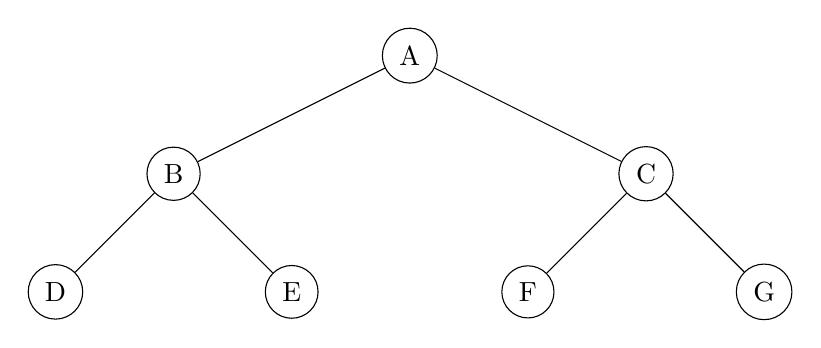
\begin{tikzpicture}[level/.style={sibling distance=60mm/#1}]
\node [circle,draw] (root) {A}
    child {
        node [circle,draw] (left) {B}
        child {
            node [circle,draw] (left-left) {D}
        }
        child {
            node [circle,draw] (left-right) {E}
        }
    }
    child {
        node [circle,draw] (right) {C}
        child {
            node [circle,draw] (right-left) {F}
        }
        child {
            node [circle,draw] (right-right) {G}
        }
    };
\end{tikzpicture}
\caption{二叉树的结构图}
\label{fig:binary_tree}
\end{figure}

\section{图的实现与测试}
\subsection{图的基本概念}
图是一种由顶点和边组成的结构,支持插入顶点、插入边、遍历等操作。

\subsection{图的实现}
使用邻接矩阵和邻接表实现图。以下是关键操作的伪代码:

\begin{verbatim}
// 插入顶点操作伪代码
void insertVertex(Graph &graph, VertexType vertex) {
    if (graph.vertexCount >= MAX_VERTEX) {
        throw "Graph is full";
    }
    graph.vertices[graph.vertexCount++] = vertex;
}
\end{verbatim}

\subsection{图的测试}
设计测试用例并分析测试结果,如下表所示:

\begin{table}
\centering
\begin{tabular}{|c|c|c|c|}
\hline
操作类型 & 输入数据 & 预期输出 & 实际输出 \\ \hline
插入顶点 & 顶点A & 成功 & 成功 \\ \hline
插入边 & 边A-B & 成功 & 成功 \\ \hline
遍历 & 深度优先 & A,B,C & A,B,C \\ \hline
\end{tabular}
\caption{图测试结果}
\label{tab:graph_test}
\end{table}

\begin{figure}
\centering
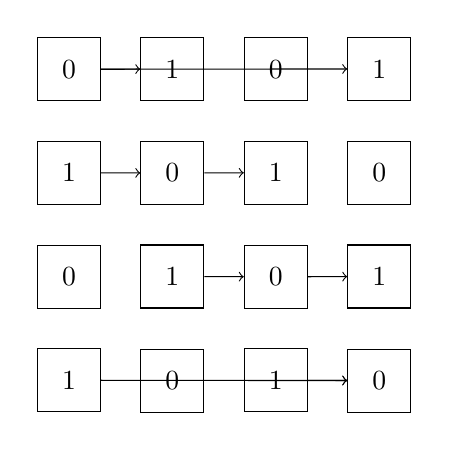
\begin{tikzpicture}
    \matrix (m) [matrix of nodes, nodes={draw, minimum size=8mm}, row sep=0.5cm, column sep=0.5cm] {
        0 & 1 & 0 & 1 \\
        1 & 0 & 1 & 0 \\
        0 & 1 & 0 & 1 \\
        1 & 0 & 1 & 0 \\
    };
    \draw[->] (m-1-1) -- (m-1-2);
    \draw[->] (m-1-1) -- (m-1-4);
    \draw[->] (m-2-1) -- (m-2-2);
    \draw[->] (m-2-2) -- (m-2-3);
    \draw[->] (m-3-2) -- (m-3-3);
    \draw[->] (m-3-3) -- (m-3-4);
    \draw[->] (m-4-1) -- (m-4-4);
    \draw[->] (m-4-3) -- (m-4-4);
\end{tikzpicture}
\caption{邻接矩阵示意图}
\label{fig:adj_matrix}
\end{figure}

\begin{figure}
\centering
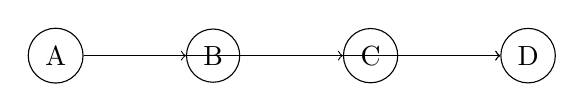
\begin{tikzpicture}
    \node[draw, circle] (A) at (0, 0) {A};
    \node[draw, circle] (B) at (2, 0) {B};
    \node[draw, circle] (C) at (4, 0) {C};
    \node[draw, circle] (D) at (6, 0) {D};
    
    \draw[->] (A) -- (B);
    \draw[->] (A) -- (D);
    \draw[->] (B) -- (C);
    \draw[->] (C) -- (D);
\end{tikzpicture}
\caption{邻接表示意图}
\label{fig:adj_list}
\end{figure}

\section{实验总结}
\subsection{实验结果总结}
通过本次实验,我们成功实现了线性表、树、图的基本操作,并进行了详细的测试。

\subsection{实验中的问题与解决方案}
在实现过程中,我们遇到了一些问题,如内存管理、边界条件处理等,通过调试和优化,最终解决了这些问题。

\subsection{未来工作展望}
未来可以进一步优化数据结构的性能,并扩展更多功能,如支持并发操作、动态调整大小等。

\section{参考文献}
\begin{itemize}
    \item 《数据结构与算法分析》 - Mark Allen Weiss
    \item 《算法导论》 - Thomas H. Cormen
\end{itemize}

\section{附录}
\subsection{源代码}
提供完整的源代码(线性表、树、图的实现)。

\subsection{测试数据}
提供测试用例的详细数据。

\end{document}